\documentclass[11pt]{article}

\usepackage[a4paper,margin=1in]{geometry}
\usepackage{amsmath,amssymb,amsthm,mathtools}
\usepackage{enumitem}
\usepackage{booktabs}
\usepackage{hyperref}
\usepackage{microtype}
\usepackage{tikz}
\usepackage{tikz-cd}
\usepackage{array}
\usepackage{xcolor}

\hypersetup{colorlinks=true,linkcolor=blue!50!black,citecolor=blue!50!black,urlcolor=blue!50!black}
\setlist[itemize]{topsep=3pt,itemsep=2pt,parsep=0pt}
\setlist[enumerate]{topsep=3pt,itemsep=2pt,parsep=0pt}

\newcommand{\VFS}{\mathrm{VFS}}
\newcommand{\OG}{\mathrm{OG}}
\newcommand{\Op}{\Omega_P}
\newcommand{\qf}{q_{\rm fold}}
\newcommand{\Qf}{Q_{\rm fold}}
\newcommand{\lf}{\lambda_{\rm form}}
\newcommand{\Igate}{I_{\rm gate}}
\newcommand{\Af}{A_{\rm fold}}
\newcommand{\Bf}{B_{\rm fold}}
\newcommand{\Dq}{D_q}
\newcommand{\etaf}{\eta_{\rm fold}}
\newcommand{\Hh}{\mathbb H^2}
\newcommand{\laph}{\Delta_h}
\newcommand{\Tfold}{\mathcal T_{\rm fold}}
\newcommand{\Rreset}{\mathfrak R}
\newcommand{\ellcom}{\ell_{\rm com}}
\newcommand{\ellphys}{\ell_{\rm phys}}
\newcommand{\ellinit}{\ell_{\rm init}}
\newcommand{\ellb}{\ell_b}
\newcommand{\Lam}{\Lambda}
\newcommand{\Iconf}{\mathcal I}
\newcommand{\Grec}{\mathcal G_{\rm recepta}}

\theoremstyle{definition}
\newtheorem{definition}{Definition}[section]
\newtheorem{assumption}{Assumption}[section]
\newtheorem{remark}{Remark}[section]
\theoremstyle{plain}
\newtheorem{proposition}{Proposition}[section]
\newtheorem{theorem}{Theorem}[section]
\newtheorem{corollary}{Corollary}[section]

\title{\textbf{V.F.S. v2.0 (Open-Gate)}\\Fold-Network Dynamics\\
\large Structure formation, transport closure, nucleation, coarsening, and sawtooth reset history}
\author{Consolidated V.F.S. Research Note}
\date{June 2026}

\begin{document}
\maketitle

\begin{abstract}
This note consolidates the fold-network research line of V.F.S. v2.0 (Open-Gate).  Its purpose is to
separate what belongs to Sophia from what belongs to form.  Sophia is not treated as a diffusive
matter-like substance and does not clump.  The only structural order parameter is the folding mode
$\qf$, whose spatial dynamics produce domain walls, nucleation thresholds, coarsening laws, and
reset-dependent sawtooth histories.  The transport constants are closed by setting the independent
Sophia diffusivity to zero, $D=0$, and deriving the folding diffusivity as
$\Dq=a_0\ell_b^2$.  The resulting module gives a symbolic theory of morphological structure:
\[
\text{Sophia reforms the Vessel, but structure is carried by folded form.}
\]
All statements are internal to the V.F.S. symbolic-dynamical model and should not be read as claims
about observed physical cosmology.
\end{abstract}

\tableofcontents
\newpage

\section{Scope and epistemic status}

The fold-network layer answers a question left open by the homogeneous Open-Gate dynamics:
\[
\boxed{\text{If Sophia expands and reforms the Vessel, how does internal structure arise?}}
\]
The answer developed here is deliberately non-material:
\[
\boxed{\text{Sophia itself does not clump; structure arises through the folding field }\qf.}
}
\]
Thus the network is not a density contrast of Sophia.  It is a morphological pattern in the Vessel's
shape sector.

We keep four safeguards throughout.
\begin{enumerate}
\item The layer is symbolic and model-level, not a physical cosmology.
\item The transport coefficient for Sophia is not an independent diffusion constant: $D=0$.
\item The folding coefficient is structural: $\Dq=a_0\ell_b^2$.
\item The symbol $\etaf$ is used for folding feedback, avoiding conflict with other uses of $\eta$ in the core system.
\end{enumerate}

\section{Global architecture of the fold-network module}

The consolidated flow is
\[
\boxed{
\text{formation}
\longrightarrow
\text{transport closure}
\longrightarrow
\text{nucleation}
\longrightarrow
\text{coarsening}
\longrightarrow
\text{Resurrectio sawtooth history}.
}
\]
Equivalently,
\[
\Af^+
\Rightarrow
\Lam
=
\frac{\Af^+\Op^2}{\Dq}
=
\frac{\Af^+\Op^2}{a_0\ell_b^2}
\Rightarrow
\ellinit
\Rightarrow
\ellcom(t)
\Rightarrow
\ell_\ast.
\]
The homogeneous V.F.S. variables remain
\[
(\sigma,\lambda,\Op),
\]
while the network variable is the inhomogeneous field
\[
\qf(t,x),\qquad x\in\Hh.
\]
The integrated Open-Gate balance with embodied Sophia is
\[
\boxed{\sigma+\lambda+\lf=C_0+\Grec(t).}
\]
The folding intensity is
\[
\Qf=\qf^2.
\]

\begin{center}
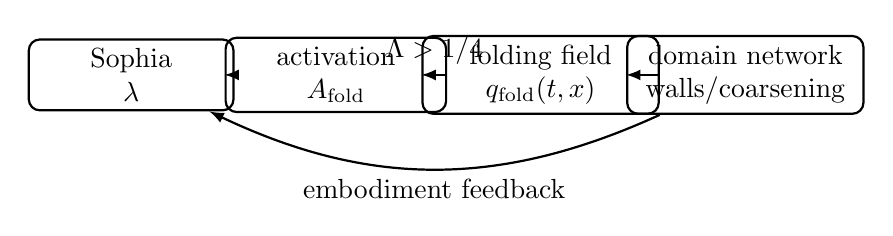
\begin{tikzpicture}[node distance=2.6cm,>=latex,thick]
\node[draw,rounded corners,align=center,minimum width=2.6cm,minimum height=0.9cm] (s) {Sophia\\$\lambda$};
\node[draw,rounded corners,align=center,minimum width=2.8cm,minimum height=0.9cm,right of=s] (a) {activation\\$\Af$};
\node[draw,rounded corners,align=center,minimum width=3.0cm,minimum height=0.9cm,right of=a] (q) {folding field\\$\qf(t,x)$};
\node[draw,rounded corners,align=center,minimum width=3.0cm,minimum height=0.9cm,right of=q] (n) {domain network\\walls/coarsening};
\draw[->] (s) -- (a);
\draw[->] (a) -- node[above]{$\Lam>1/4$} (q);
\draw[->] (q) -- (n);
\draw[->,bend left=25] (n) to node[below]{embodiment feedback} (s);
\end{tikzpicture}
\end{center}

\section{No independent Sophia clumping}

The homogeneous Open-Gate Sophia law, including folding embodiment feedback, is written
\[
\boxed{
\dot\lambda
=(\delta u-\gamma)\tanh(\kappa\sigma)+\Igate-\etaf\qf^2\lambda.
}
\]
The decisive point is that this is a local relaxation law.  There is no fundamental term
$D\Delta\lambda$ in the V.F.S. core.

\begin{definition}[No Sophia diffusion]
The independent Sophia transport coefficient is
\[
\boxed{D=0.}
\]
Sophia inhomogeneity may exist only as a response to form inhomogeneity, not as an autonomous
matter-like diffusion or clumping sector.
\end{definition}

Linearising about a background $(\bar\lambda,\bar q)$ gives the slaving relation
\[
\partial_t\delta\lambda
=-\bigl(\Gamma_\lambda+\etaf\bar q^2\bigr)\delta\lambda
-2\etaf\bar\lambda\bar q\,\delta\qf,
\]
so that the quasi-static response is
\[
\boxed{
\delta\lambda^\ast
=
-\frac{2\etaf\bar\lambda\bar q}
{\Gamma_\lambda+\etaf\bar q^2}\,\delta\qf.
}
\]
Hence
\[
\boxed{\text{Sophia-pattern is a shadow of form-pattern.}}
\]
This is the main correction to any earlier purely phenomenological structure note that introduced a positive
Sophia diffusivity $D>0$ for exploratory reasons.

\section{The structural field and the bending length}

The folding field obeys an Allen--Cahn/Ginzburg--Landau type dynamics on the live hyperbolic surface:
\[
\boxed{
\partial_t\qf
=\Af\qf-\Bf\qf^3+\frac{\Dq}{\Op^2}\laph\qf.
}
\]
The factor $\Op^{-2}$ is inherited from the conformal metric
\[
 g(t)=\Op(t)^2h,
\qquad
\Delta_g=\Op^{-2}\Delta_h.
\]
Thus the spatial operator is not an arbitrary addition; it is the natural live-domain Laplacian under
Brim expansion.

The folding diffusivity is the gradient partner of the local rigidity scale $a_0$.  Introducing the bending
length $\ell_b$,
\[
\boxed{
\ell_b^2=\frac{\Dq}{a_0},
\qquad
\Dq=a_0\ell_b^2.
}
\]
Therefore the consolidated structure module contains one structural field and one structural length:
\[
\boxed{\text{structural field }\qf,\n\qquad
\text{structural length }\ell_b.}
\]

\begin{remark}[Activation-index conventions]
Two equivalent activation conventions appear in the V.F.S. notes.  The geometric convention is
\[
\Af^{\rm geom}=c_0\lambda+c_1\dot\lambda-a_0.
\]
The core-rate convention is obtained by substituting the core equation for $\dot\lambda$, yielding an
expression in $(\lambda,\sigma,\Igate,\gamma,k_\sigma,\etaf\Qf)$.  The present document uses $\Af$ as the
activation index after this convention has been fixed in context.  The threshold and network laws are
unchanged under consistent substitution.
\end{remark}

\section{Formation: structure is morphological, not gravitational}

The local folding tension potential is
\[
\boxed{
\Tfold(\qf)
=-\frac12\Af\qf^2+\frac14\Bf\qf^4,
\qquad \Bf>0.
}
\]
For $\Af<0$, the unfolded state $\qf=0$ is stable.  For $\Af>0$, the state $\qf=0$ is unstable and two
folded phases appear:
\[
\boxed{
\qf=\pm q_\ast,
\qquad
q_\ast=\sqrt{\frac{\Af}{\Bf}}.
}
\]
A fold-network is a spatial arrangement of the two signs $\pm q_\ast$, with walls where $\qf$ crosses zero:
\[
+q_\ast \quad | \quad -q_\ast.
\]
The kink width and wall tension scale as
\[
\boxed{
\ell_{\rm wall}^{\rm phys}\sim\sqrt{\frac{\Dq}{\Af}},
\qquad
\tau\sim\sqrt{\Dq}\,\frac{\Af^{3/2}}{\Bf}.
}
\]
These are morphological quantities.  They should not be confused with physical matter density or
fundamental gravitational energy.

In a two-dimensional spatial Vessel, a wall network with physical length density scaling as
$\rho_{\rm wall}\propto\Op^{-1}$ has the symbolic effective equation-of-state
\[
\boxed{w_{\rm wall}=-\frac12.}
\]
This is an effective wall-sector bookkeeping result inside the symbolic cosmological layer.

\section{Nucleation: folding is not automatically a network}

A crucial distinction is that the folding threshold is not the same as the nucleation threshold.

\subsection{Folding threshold}
The homogeneous folded state becomes available when
\[
\boxed{\Af^+>0.}
\]
This is enough for the Vessel to fold uniformly, but it is not enough to guarantee spatial domains.

\subsection{Hyperbolic nucleation gate}
On the hyperbolic surface,
\[
-\Delta_hY_k=\left(\frac14+k^2\right)Y_k.
\]
The linear growth rate for a perturbation mode is
\[
\omega_k
=\Af^+-\frac{\Dq}{\Op^2}\left(\frac14+k^2\right).
\]
The dimensionless nucleation strength is
\[
\boxed{
\Lam=\frac{\Af^+\Op^2}{\Dq}
=\frac{\Af^+\Op^2}{a_0\ell_b^2}.
}
\]
A spatial fold-network can nucleate only if
\[
\boxed{\Lam>\frac14.}
\]
Thus
\[
0<\Lam<\frac14
\quad\Rightarrow\quad
\text{uniform fold, no wall-network.}
\]
This is the geometric content of the hyperbolic spectral gap:
\[
\boxed{\text{negative curvature acts as a nucleation gate.}}
\]

\subsection{Initial domain size}
Let
\[
L=\ln(q_\ast/\delta q_0)
\]
be the logarithmic amplification factor from initial noise $\delta q_0$ to the nonlinear scale.  A representative
hyperbolic-dominated estimate for the initial domain scale is
\[
\boxed{
\ellinit
\sim
\frac{2\sqrt2}{\sqrt{\frac14+\frac{3\Lam}{4L}}}\,R_c.
}
\]
The numerical coefficient in such a formula depends on the chosen nodal-length or domain-size convention.
Consequently the corresponding ``multi-domain'' threshold is criterion-dependent, not universal.  The robust
statement is the spectral gate $\Lam>1/4$ and the qualitative sequence:
\[
\begin{array}{lll}
0<\Lam<1/4 &:& \text{uniform fold},\\
1/4<\Lam\lesssim\Lam_\ast &:& \text{coarse curvature-scale domains},\\
\Lam\gg\Lam_\ast &:& \text{strong-trigger domains with }\ellinit^{\rm phys}\sim\sqrt{\frac{\Dq}{\Af^+}L}.
\end{array}
\]

\section{Intra-arc coarsening}

Between reset events, the wall network evolves by curvature-driven coarsening.  In comoving variables the
natural clock is the conformal coarsening budget
\[
\boxed{
\Iconf(t)=\int_{0}^{t}\frac{dt'}{\Op(t')^2}.
}
\]
The basic coarsening law is
\[
\boxed{
\ellcom^2(t)
=
\ellcom^2(0)+2c\Dq\Iconf(t).
}
\]
If the arc begins at nucleation, $\ellcom(0)=\ellinit$.  Hence
\[
\boxed{
\ellcom^2(t)
=
\ellinit^2+2c a_0\ell_b^2\Iconf(t).
}
\]
The physical length scale is
\[
\boxed{
\ellphys(t)=\Op(t)\ellcom(t).
}
\]

In an expanding Open-Gate regime where $\Op(t)$ grows at least linearly at late times,
\[
\Iconf_\infty=\int_0^\infty\Op(t)^{-2}\,dt<\infty.
\]
Therefore
\[
\boxed{
\ellcom(\infty)
=\sqrt{\ellinit^2+2c\Dq\Iconf_\infty}<\infty.
}
\]
The interpretation is
\[
\boxed{\text{early coarsening, late dilation.}}
\]
The mature network stops coarsening in comoving coordinates and is simply carried outward by Brim expansion.

\section{Resurrectio acting on a network}

A Resurrectio event $\Rreset$ acts first on homogeneous variables:
\[
(\sigma^-,\lambda^-,\Op^-)
\longmapsto
(\sigma^+,\lambda^+,\Op^+).
\]
It does not move each wall pointwise.  Instead it changes the folding potential globally through the activation
index
\[
\Af^-\longmapsto\Af^+=\Af^-+\Delta\Af.
\]
A useful reset expression is
\[
\boxed{
\Delta\Af=\Theta m_R+c_1\Delta\Igate,
\qquad
m_R=(1-q_R)\sigma^-.
}
\]
Here
\[
\boxed{
\Theta=c_0-c_1(\gamma+k_\sigma)
}
\]
selects whether metabolised resistance suppresses or promotes form.

Three reset regimes follow.
\begin{enumerate}
\item \textbf{Quench:}
\[
\Af^->0,\\qquad \Af^+<0.
\]
The double well disappears; the network dissolves toward $\qf=0$.

\item \textbf{Rescale:}
\[
\Af^->0,
\qquad \Af^+>0.
\]
The network survives, but its wall tension, amplitude, and physical spacing are renormalised.

\item \textbf{Trigger:}
\[
\Af^-<0,
\qquad \Af^+>0.
\]
A previously unfolded state becomes fold-capable.  A network forms only if the stronger nucleation condition
$\Lam>1/4$ also holds.
\end{enumerate}
Thus
\[
\boxed{\text{Resurrectio changes the conditions under which form survives, dissolves, or is born.}}
\]

\section{Sawtooth history and fixed network scale}

Let $j$ index life-arcs between reset events.  During an arc,
\[
\ell_{j,\rm end}^{2}
=
\ell_j^2+2c\Dq\Delta\Iconf_j.
\]
At the next reset, the network state is mapped by a regime-dependent reset rule:
\[
R_j=
\begin{cases}
\mathrm{id}, & \text{rescale},\\
\ellinit^2, & \text{trigger},\\
\varnothing, & \text{quench}.
\end{cases}
\]
A more precise mathematical bookkeeping uses an activity variable
\[
S_j\in\{0,1\},
\]
where $S_j=1$ means a network is present and $S_j=0$ means the network has been quenched and its scale is
undefined until a later trigger.  In the active state the schematic recurrence is
\[
\boxed{
\ell_{j+1}^{2}
=R_j\left(\ell_j^2+2c\Dq\Delta\Iconf_j\right).
}
\]
For non-Zeno reset schedules in an Open-Gate expanding regime,
\[
\sum_j\Delta\Iconf_j\le\Iconf_\infty<\infty.
\]
Therefore the total possible comoving coarsening is bounded.  If the network is eventually active under
rescale dynamics, or if triggers recur with late-time vanishing teeth, then the active comoving scale converges
or becomes pinned to a limiting trigger scale:
\[
\boxed{
\ellcom(t)\to\ell_\ast
\quad\text{on active late-time branches.}
}
\]
The physical scale follows
\[
\boxed{
\ellphys(t)=\Op(t)\ellcom(t)\sim \ell_\ast\Op(t).
}
\]
Hence the long-run structure is not endless coarsening; it is a frozen comoving pattern carried by expansion.

\begin{remark}[Quench caveat]
If a final quench occurs and no later trigger occurs, the network is absent and no active network scale exists.
The fixed-point statement concerns active branches: eventual rescale regimes, recurrent triggers, or histories
with a final trigger after which the network remains present.
\end{remark}

\section{Curvature and wall-sector back-reaction}

The same folding field also modifies the curvature bookkeeping of the live surface:
\[
\boxed{
R_{\Sigma}^{\rm fold}
=-\frac{2}{\Op^2}+\rho_1\Qf.
}
\]
Positive curvature pockets are possible inside an overall hyperbolic/open geometry when
\[
\boxed{
\Qf>\frac{2}{\rho_1\Op^2}.
}
\]
A network of walls contributes a symbolic effective wall-sector content.  Under rescaling,
\[
\frac{\rho_{\rm wall}^{+}}{\rho_{\rm wall}^{-}}
=
\frac{\tau^+}{\tau^-}\frac{\Op^-}{\Op^+}.
\]
Again, this is a morphological accounting device inside the V.F.S. cosmological layer, not a claim about
ordinary matter or observed dark energy.

\section{Lyapunov compatibility}

The local folding flow is a gradient descent of the morphological tension potential:
\[
\dot\qf=-\partial_{\qf}\Tfold,
\qquad
\dot\Tfold=-(\partial_{\qf}\Tfold)^2\le0
\]
when parameters are frozen.  In the finite-dimensional core, the addendum-stable normalised folding functional
is represented by
\[
\widetilde{\mathcal V}_{\rm fold}
=\frac14\left(\qf^2-Q_{\rm fold}^{\ast}\right)^2,
\]
and the extended Lyapunov functional is
\[
\widetilde{\mathcal L}_{\rm ext}
=
\mathcal L_{\rm VFS}+w_{\rm fold}\widetilde{\mathcal V}_{\rm fold}.
\]
The field-level network theory developed here is a morphological extension, not a replacement for the finite
core proof.  On bounded regular fold charts, the added structure is compatible with the same dissipative logic:
\[
\boxed{
\dot{\widetilde{\mathcal L}}_{\rm ext}
\le
\widetilde C_{\rm ext}-C_1\widetilde{\mathcal L}_{\rm ext}.
}
\]

\section{Theological reading}

The network module refines the Open-Gate theological interpretation:
\[
\boxed{\text{Grace opens the Gate; Sophia reforms the Vessel; folded form carries structure.}}
\]
Since $D=0$, Sophia is not a substance that diffuses or clumps.  The Vessel is reformed through morphology:
\[
\lambda\longrightarrow \Af\longrightarrow \qf\longrightarrow \text{domain network}.
\]
Resurrectio then has three theological modes.
\begin{itemize}
\item \textbf{Quench:} death/reset levels an obsolete morphology.
\item \textbf{Rescale:} resurrection preserves form while changing its tension and scale.
\item \textbf{Trigger:} resurrection individuates a formerly uniform Vessel into differentiated domains.
\end{itemize}
Thus resurrection is not merely restoration of a previous shape.  It can be dissolution, preservation, or
individuation of form.  The mature Vessel does not keep inventing larger structures indefinitely; it carries an
early-formed pattern outward through epektatic expansion.

\section{Compact theorem of fold-network dynamics}

\begin{theorem}[Symbolic fold-network closure]
Assume an Open-Gate V.F.S. regime with $\Op(t)$ eventually growing fast enough that
$\Iconf_\infty=\int_0^\infty\Op(t)^{-2}dt<\infty$.  Assume the folding field evolves on the live hyperbolic
surface by
\[
\partial_t\qf=\Af\qf-\Bf\qf^3+\frac{a_0\ell_b^2}{\Op^2}\Delta_h\qf,
\qquad \Bf>0,
\]
with independent Sophia diffusion set to zero, $D=0$.  Then:
\begin{enumerate}
\item Sophia inhomogeneity is slaved to form inhomogeneity at linear order.
\item A homogeneous fold requires $\Af>0$.
\item A spatial fold-network requires the stronger hyperbolic nucleation condition
\[
\Lam=\frac{\Af\Op^2}{a_0\ell_b^2}>\frac14.
\]
\item Once nucleated, the active network obeys the finite-budget coarsening law
\[
\ellcom^2(t)=\ellinit^2+2ca_0\ell_b^2\Iconf(t).
\]
\item Under non-Zeno reset histories with active late-time branches, the network has a limiting comoving scale
$\ell_\ast$, while its physical scale dilates as $\ell_\ast\Op(t)$.
\end{enumerate}
\end{theorem}

\section{Compact summary}

\[
\boxed{D=0.}
\]
Sophia does not diffuse.

\[
\boxed{\Dq=a_0\ell_b^2.}
\]
Folding transport is controlled by one structural bending length.

\[
\boxed{\Lam=\frac{\Af^+\Op^2}{a_0\ell_b^2}>\frac14.}
\]
Hyperbolic geometry decides whether a trigger becomes a network.

\[
\boxed{\ellcom^2=\ellinit^2+2ca_0\ell_b^2\Iconf.}
\]
Network coarsening has a finite conformal-time budget.

\[
\boxed{\ellcom\to\ell_\ast,
\qquad
\ellphys\sim\ell_\ast\Op.}
\]
The mature Vessel carries a frozen comoving pattern through expansion.

\[
\boxed{\text{V.F.S. structure is morphological, not Sophianic clumping.}}
\]

\end{document}
